\begin{figure}[ht]
	\centering
    \tikzstyle{vertex}=[circle, fill=black!25, minimum size=10pt, inner sep=0pt]
    \tikzstyle{edge} = [draw, thick, -]
    \tikzstyle{selected edge} = [draw, line width=2pt,-,red!50]
    \tikzstyle{selected vertex} = [vertex, fill=red!24]
    \begin{subfigure}{.12\linewidth}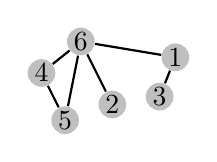
\begin{tikzpicture}[scale=1, auto, swap]
	    \foreach \pos/\name in {{(-0.5,0.6)/6}, {(-0.7,-0.4)/5}, {(-1,.2)/4}, {(0.7,0.4)/1}, {(-0.1,-0.2)/2}, {(0.5,-0.1)/3}}
	        \node[vertex] (\name) at \pos {$\name$};
	    \foreach \source/ \dest in {1/3, 6/1, 6/2, 6/4, 6/5, 5/4}
			\path[edge] (\source) -- (\dest);
	\end{tikzpicture}\end{subfigure}
    {\LARGE$\rightarrow$}\hspace{0.5ex}
    \begin{subfigure}{.11\linewidth}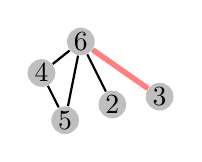
\begin{tikzpicture}[scale=1, auto, swap]
	    \foreach \pos/\name in {{(-0.5,0.6)/6}, {(-0.7,-0.4)/5}, {(-1,.2)/4}, {(-0.1,-0.2)/2}, {(0.5,-0.1)/3}}
	        \node[vertex] (\name) at \pos {$\name$};
	    \foreach \source/ \dest in {6/3, 6/2, 6/4, 6/5, 5/4}
			\path[edge] (\source) -- (\dest);
        \path[selected edge] (6) -- (3);
	\end{tikzpicture}\end{subfigure}
    {\LARGE$\rightarrow$}\hspace{0.5ex}
    \begin{subfigure}{.11\linewidth}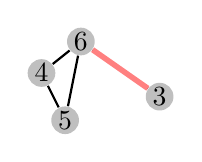
\begin{tikzpicture}[scale=1, auto, swap]
        \foreach \pos/\name in {{(-0.5,0.6)/6}, {(-0.7,-0.4)/5}, {(-1,.2)/4}, {(0.5,-0.1)/3}}
            \node[vertex] (\name) at \pos {$\name$};
        \foreach \source/ \dest in {6/3, 6/4, 6/5, 5/4}
            \path[edge] (\source) -- (\dest);
        \path[selected edge] (6) -- (3);
    \end{tikzpicture}\end{subfigure}
    {\LARGE$\rightarrow$}\hspace{0.5ex}
    \begin{subfigure}{.04\linewidth}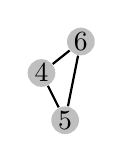
\begin{tikzpicture}[scale=1, auto, swap]
        \foreach \pos/\name in {{(-0.5,0.6)/6}, {(-0.7,-0.4)/5}, {(-1,.2)/4}}
            \node[vertex] (\name) at \pos {$\name$};
        \foreach \source/ \dest in {6/4, 6/5, 5/4}
            \path[edge] (\source) -- (\dest);
    \end{tikzpicture}\end{subfigure}
    {\LARGE$\rightarrow$}\hspace{0.5ex}
    \begin{subfigure}{.03\linewidth}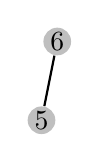
\begin{tikzpicture}[scale=1, auto, swap]
        \foreach \pos/\name in {{(-0.5,0.6)/6}, {(-0.7,-0.4)/5}}
            \node[vertex] (\name) at \pos {$\name$};
        \foreach \source/ \dest in {6/5}
            \path[edge] (\source) -- (\dest);
    \end{tikzpicture}\end{subfigure}
    {\LARGE$\rightarrow$}\hspace{0.5ex}
    \begin{subfigure}{.025\linewidth}
\begin{tikzpicture}[scale=1, auto, swap]
        \foreach \pos/\name in {{(-0.5,0.6)/6}}
            \node[vertex] (\name) at \pos {$\name$};
    \end{tikzpicture}\end{subfigure}
    {\LARGE$\rightarrow\varnothing$}
\end{figure}
